\newpage
\subsection{Potenzfunktionen}

$y=a*x^n$ mit $a=1$


\hfill \break
\textcolor{red}{n positiv und gerade}
\begin{itemize}
    \item Definitionsmenge: $O = \mathbb{R}$
    \item Wertemenge: $W = \mathbb{R}_0^{+}$
    \item streng monoton fallend in: $\mathbb{R}_0^{-}$
    \item streng monoton steigend in: $\mathbb{R}_0^{+}$
    \item Alle Grapen gehen durch folgende Punkte: $P(-1|1),P(0|0),P(1|1)$
\end{itemize}

\hfill \break
\textcolor{green}{n positiv und ungerade}
\begin{itemize}
    \item Definitionsmenge: $O = \mathbb{R}$
    \item Wertemenge: $W = \mathbb{R}$
    \item streng monoton fallend in: --
    \item streng monoton steigend in: $\mathbb{R}$
    \item Alle Grapen gehen durch folgende Punkte: $P(-1|-1),P(0|0),P(1|1)$
\end{itemize}

\hfill \break
\textcolor{blue}{n negativ und gerade}
\begin{itemize}
    \item Definitionsmenge: $O = \mathbb{R}$ ohne $\{0\}$
    \item Wertemenge: $W = \mathbb{R}^{+}$
    \item streng monoton fallend in: $\mathbb{R}^{+}$
    \item streng monoton steigend in: $\mathbb{R}^{-}$
    \item Alle Grapen gehen durch folgende Punkte: $P(-1|1),P(1|1)$
    \item Asymptote: x und y Achsen $x=0$ $y=0$
\end{itemize}

\newpage
\textcolor{violet}{n negativ und gerade}
\begin{itemize}
    \item Definitionsmenge: $O = \mathbb{R}$ ohne $\{0\}$
    \item Wertemenge: $W = \mathbb{R}$ ohne $\{0\}$
    \item streng monoton fallend in: $\mathbb{R}$ ohne $\{0\}$
    \item streng monoton steigend in: --
    \item Alle Grapen gehen durch folgende Punkte: $P(-1|-1),P(1|1)$
    \item Asymptote: x und y Achsen $x=0$ $y=0$
\end{itemize}

\hfill \break
Graptische darstellung:
\hfill \break
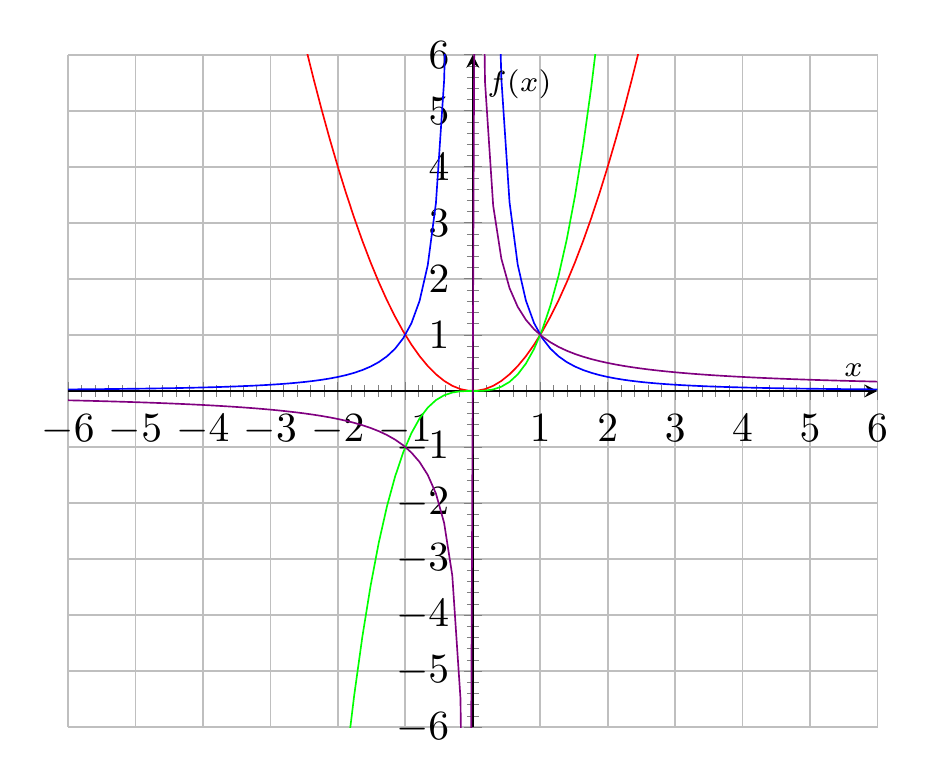
\begin{tikzpicture}[scale=1.5]
    \begin{axis}%
        [
            grid=major,
            xtick={-7,-6,...,7},
            minor x tick num=4, % 4 minor ticks => 5 subintervals
            xmin=-6,
            xmax=6,
            xlabel={\scriptsize $x$},
            axis x line=middle,
            ytick={-7,-6,...,7},
            minor y tick num=4,  % 4 minor ticks => 5 subintervals
            ymin=-6,
            ymax=6,
            ylabel={\scriptsize $f(x)$},
            axis y line=middle,
            no markers,
            samples=100,
            domain=-6:6,
        ]
        \addplot[red] (x,{1*x^2});
        \addplot[green] (x,{1*x^3});
        \addplot[blue] (x,{1*x^(-2)});
        \addplot[violet] (x,{1*x^(-1)});
    \end{axis}
\end{tikzpicture}